% Options for packages loaded elsewhere
% Options for packages loaded elsewhere
\PassOptionsToPackage{unicode}{hyperref}
\PassOptionsToPackage{hyphens}{url}
%
\documentclass[
  ignorenonframetext,
  aspectratio=169,
]{beamer}
\newif\ifbibliography
\usepackage{pgfpages}
\setbeamertemplate{caption}[numbered]
\setbeamertemplate{caption label separator}{: }
\setbeamercolor{caption name}{fg=normal text.fg}
\beamertemplatenavigationsymbolsempty
% remove section numbering
\setbeamertemplate{part page}{
  \centering
  \begin{beamercolorbox}[sep=16pt,center]{part title}
    \usebeamerfont{part title}\insertpart\par
  \end{beamercolorbox}
}
\setbeamertemplate{section page}{
  \centering
  \begin{beamercolorbox}[sep=12pt,center]{section title}
    \usebeamerfont{section title}\insertsection\par
  \end{beamercolorbox}
}
\setbeamertemplate{subsection page}{
  \centering
  \begin{beamercolorbox}[sep=8pt,center]{subsection title}
    \usebeamerfont{subsection title}\insertsubsection\par
  \end{beamercolorbox}
}
% Prevent slide breaks in the middle of a paragraph
\widowpenalties 1 10000
\raggedbottom
\usepackage{iftex}
\ifPDFTeX
  \usepackage[T1]{fontenc}
  \usepackage[utf8]{inputenc}
  \usepackage{textcomp} % provide euro and other symbols
\else % if luatex or xetex
  \usepackage{unicode-math} % this also loads fontspec
  \defaultfontfeatures{Scale=MatchLowercase}
  \defaultfontfeatures[\rmfamily]{Ligatures=TeX,Scale=1}
\fi
\usepackage{lmodern}

\usetheme[]{metropolis}
\usecolortheme[]{default}
\usefonttheme[]{default}
\ifPDFTeX\else
  % xetex/luatex font selection
\fi
% Use upquote if available, for straight quotes in verbatim environments
\IfFileExists{upquote.sty}{\usepackage{upquote}}{}
\IfFileExists{microtype.sty}{% use microtype if available
  \usepackage[]{microtype}
  \UseMicrotypeSet[protrusion]{basicmath} % disable protrusion for tt fonts
}{}
\makeatletter
\@ifundefined{KOMAClassName}{% if non-KOMA class
  \IfFileExists{parskip.sty}{%
    \usepackage{parskip}
  }{% else
    \setlength{\parindent}{0pt}
    \setlength{\parskip}{6pt plus 2pt minus 1pt}}
}{% if KOMA class
  \KOMAoptions{parskip=half}}
\makeatother


\usepackage{longtable,booktabs,array}
\usepackage{calc} % for calculating minipage widths
\usepackage{caption}
% Make caption package work with longtable
\makeatletter
\def\fnum@table{\tablename~\thetable}
\makeatother
\usepackage{graphicx}
\makeatletter
\newsavebox\pandoc@box
\newcommand*\pandocbounded[1]{% scales image to fit in text height/width
  \sbox\pandoc@box{#1}%
  \Gscale@div\@tempa{\textheight}{\dimexpr\ht\pandoc@box+\dp\pandoc@box\relax}%
  \Gscale@div\@tempb{\linewidth}{\wd\pandoc@box}%
  \ifdim\@tempb\p@<\@tempa\p@\let\@tempa\@tempb\fi% select the smaller of both
  \ifdim\@tempa\p@<\p@\scalebox{\@tempa}{\usebox\pandoc@box}%
  \else\usebox{\pandoc@box}%
  \fi%
}
% Set default figure placement to htbp
\def\fps@figure{htbp}
\makeatother





\setlength{\emergencystretch}{3em} % prevent overfull lines

\providecommand{\tightlist}{%
  \setlength{\itemsep}{0pt}\setlength{\parskip}{0pt}}



 


\makeatletter
\@ifpackageloaded{caption}{}{\usepackage{caption}}
\AtBeginDocument{%
\ifdefined\contentsname
  \renewcommand*\contentsname{Table of contents}
\else
  \newcommand\contentsname{Table of contents}
\fi
\ifdefined\listfigurename
  \renewcommand*\listfigurename{List of Figures}
\else
  \newcommand\listfigurename{List of Figures}
\fi
\ifdefined\listtablename
  \renewcommand*\listtablename{List of Tables}
\else
  \newcommand\listtablename{List of Tables}
\fi
\ifdefined\figurename
  \renewcommand*\figurename{Figure}
\else
  \newcommand\figurename{Figure}
\fi
\ifdefined\tablename
  \renewcommand*\tablename{Table}
\else
  \newcommand\tablename{Table}
\fi
}
\@ifpackageloaded{float}{}{\usepackage{float}}
\floatstyle{ruled}
\@ifundefined{c@chapter}{\newfloat{codelisting}{h}{lop}}{\newfloat{codelisting}{h}{lop}[chapter]}
\floatname{codelisting}{Listing}
\newcommand*\listoflistings{\listof{codelisting}{List of Listings}}
\makeatother
\makeatletter
\makeatother
\makeatletter
\@ifpackageloaded{caption}{}{\usepackage{caption}}
\@ifpackageloaded{subcaption}{}{\usepackage{subcaption}}
\makeatother

\usepackage{bookmark}
\IfFileExists{xurl.sty}{\usepackage{xurl}}{} % add URL line breaks if available
\urlstyle{same}
\hypersetup{
  pdftitle={Automating the Mundane: A Practitioner's System for Engineering Leverage with AI},
  pdfauthor={Mo Battah},
  hidelinks,
  pdfcreator={LaTeX via pandoc}}


\title{Automating the Mundane: A Practitioner's System for Engineering
Leverage with AI}
\subtitle{Alpine Investors \& Portfolio Companies}
\author{Mo Battah}
\date{2025-08-20}

\begin{document}
\frame{\titlepage}


\begin{frame}{Personal Systems That Scale to Business Impact}
\phantomsection\label{personal-systems-that-scale-to-business-impact}
\textbf{Mo Battah}\\
Alpine Investors \& Portfolio Companies\\
08/20/2025
\end{frame}

\begin{frame}
\end{frame}

\section{\texorpdfstring{\textbf{What This Talk is NOT
About}}{What This Talk is NOT About}}\label{what-this-talk-is-not-about}

\begin{frame}{\textbf{Future of Software Development}}
\phantomsection\label{future-of-software-development}
\begin{figure}

\begin{minipage}{0.50\linewidth}
\pandocbounded{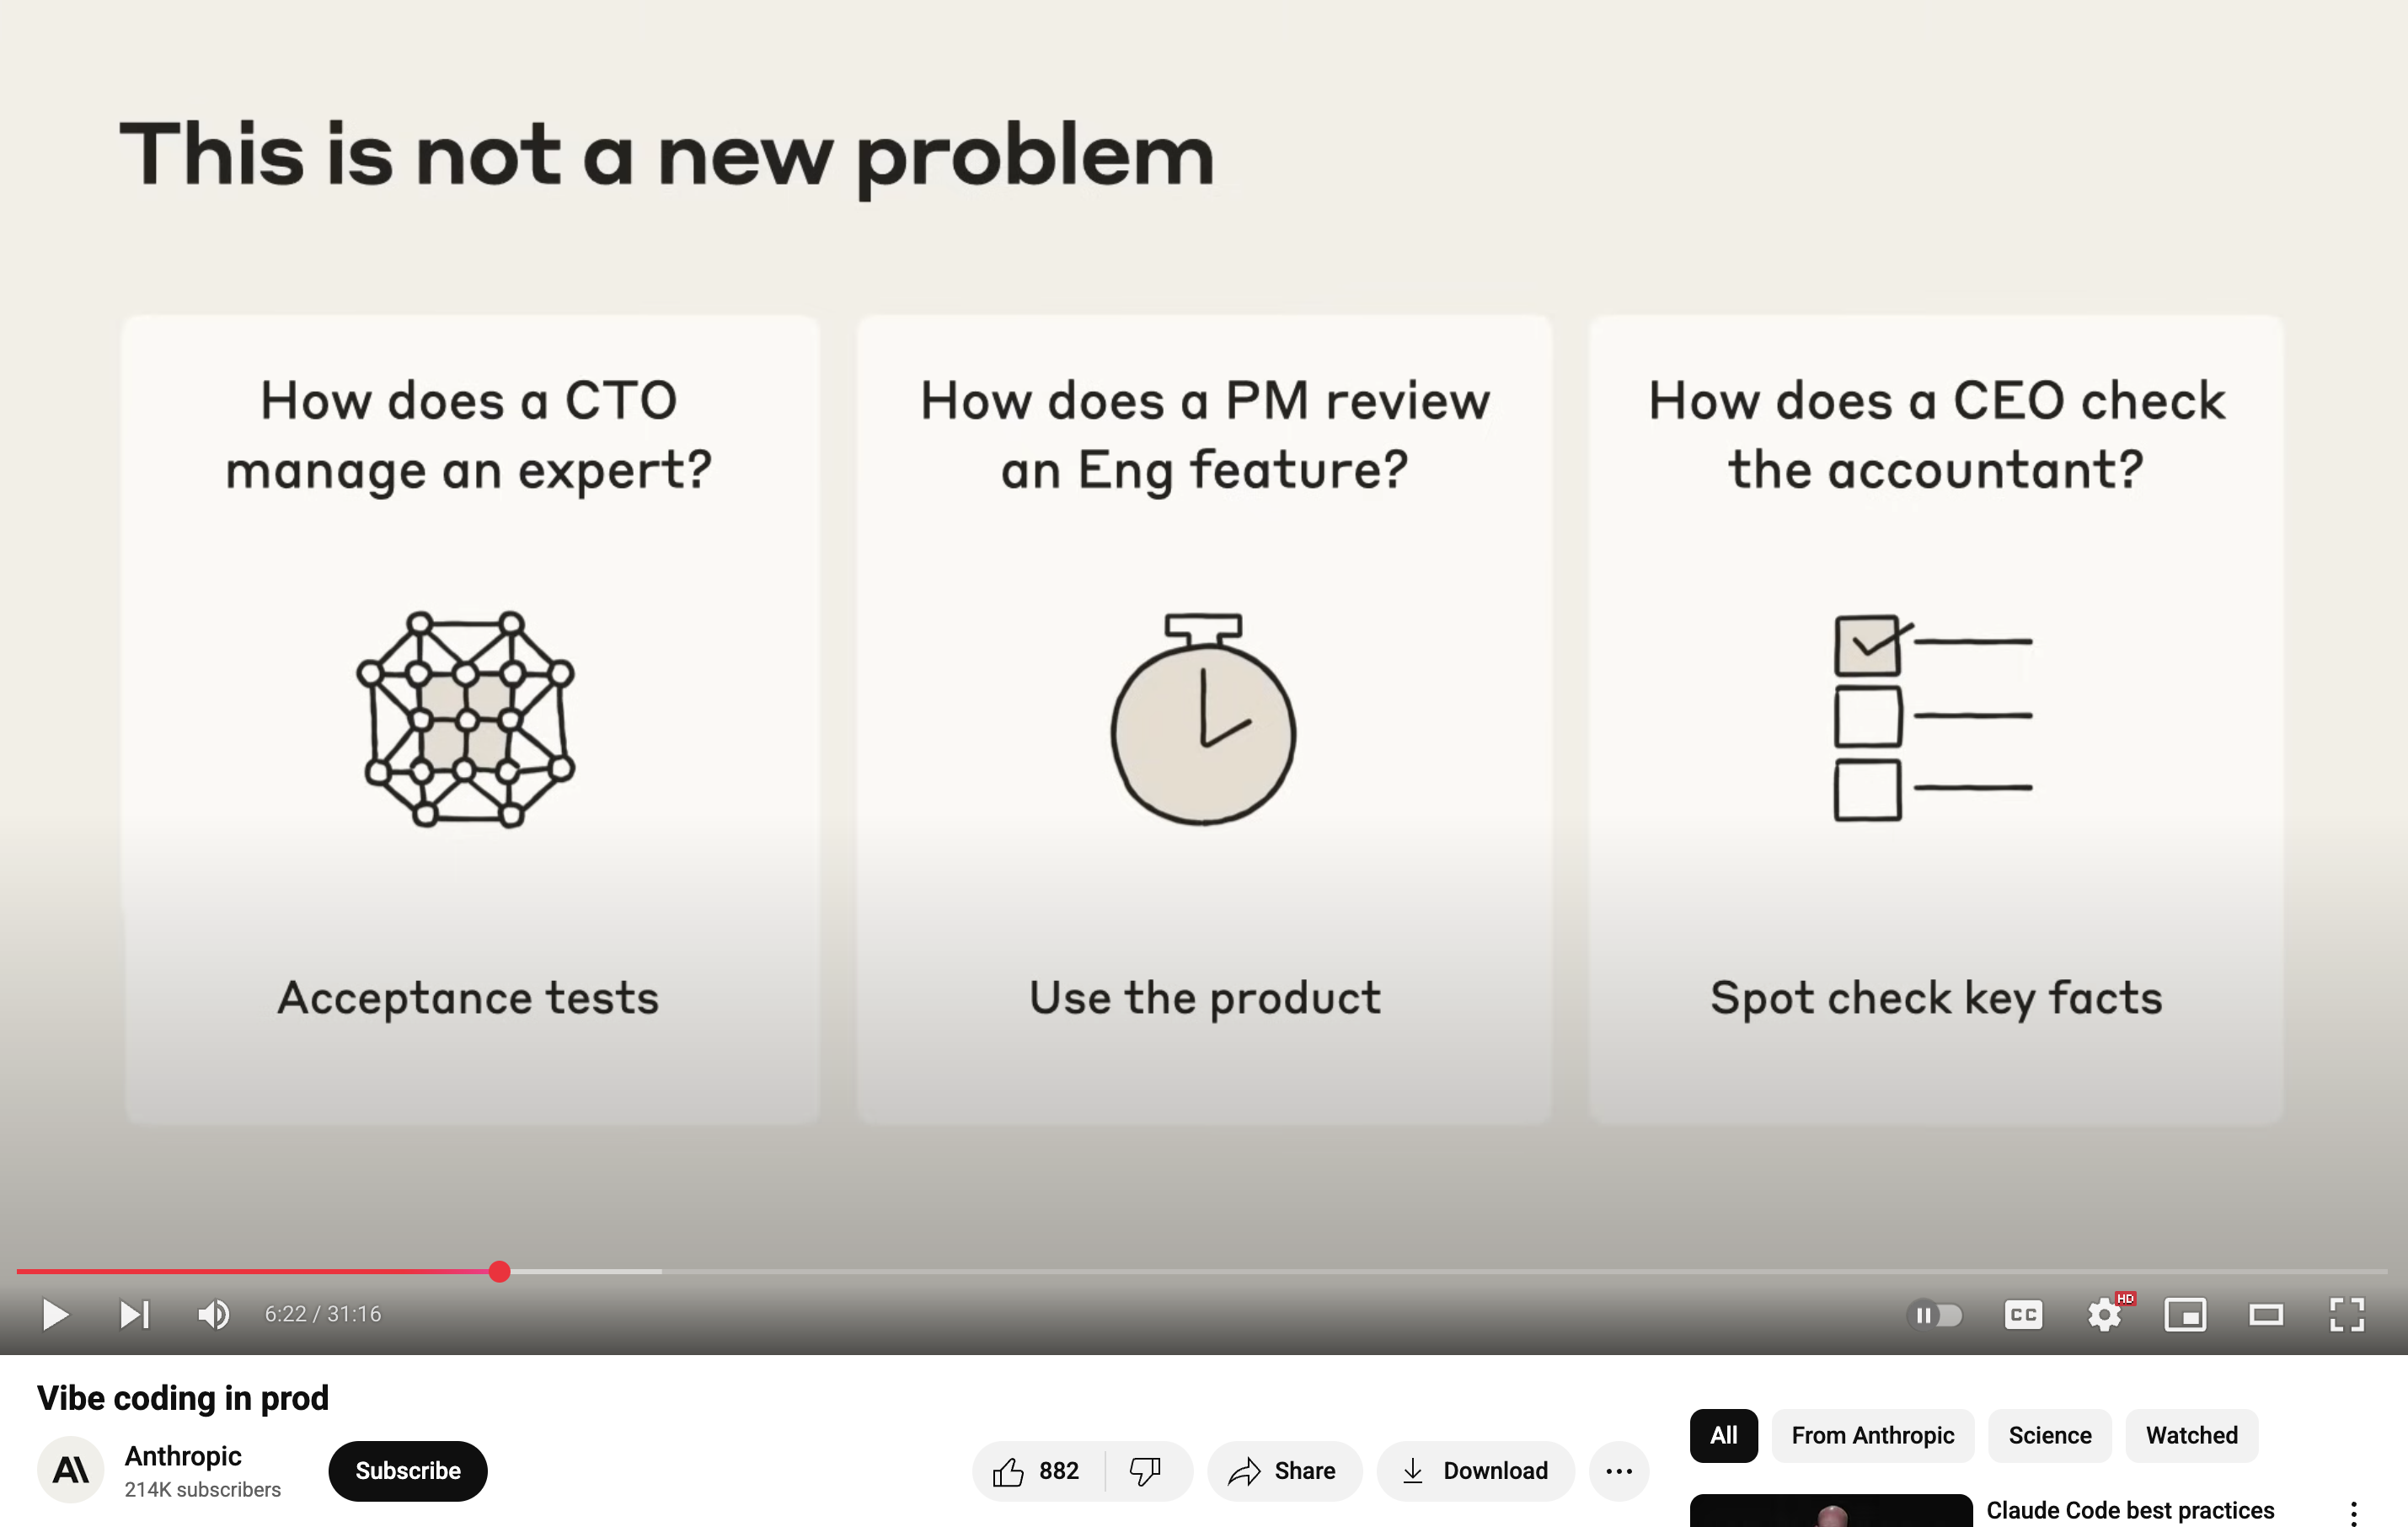
\includegraphics[keepaspectratio]{images/Anthropic Vibe Coding - How different roles review work.png}}\end{minipage}%
%
\begin{minipage}{0.50\linewidth}
\pandocbounded{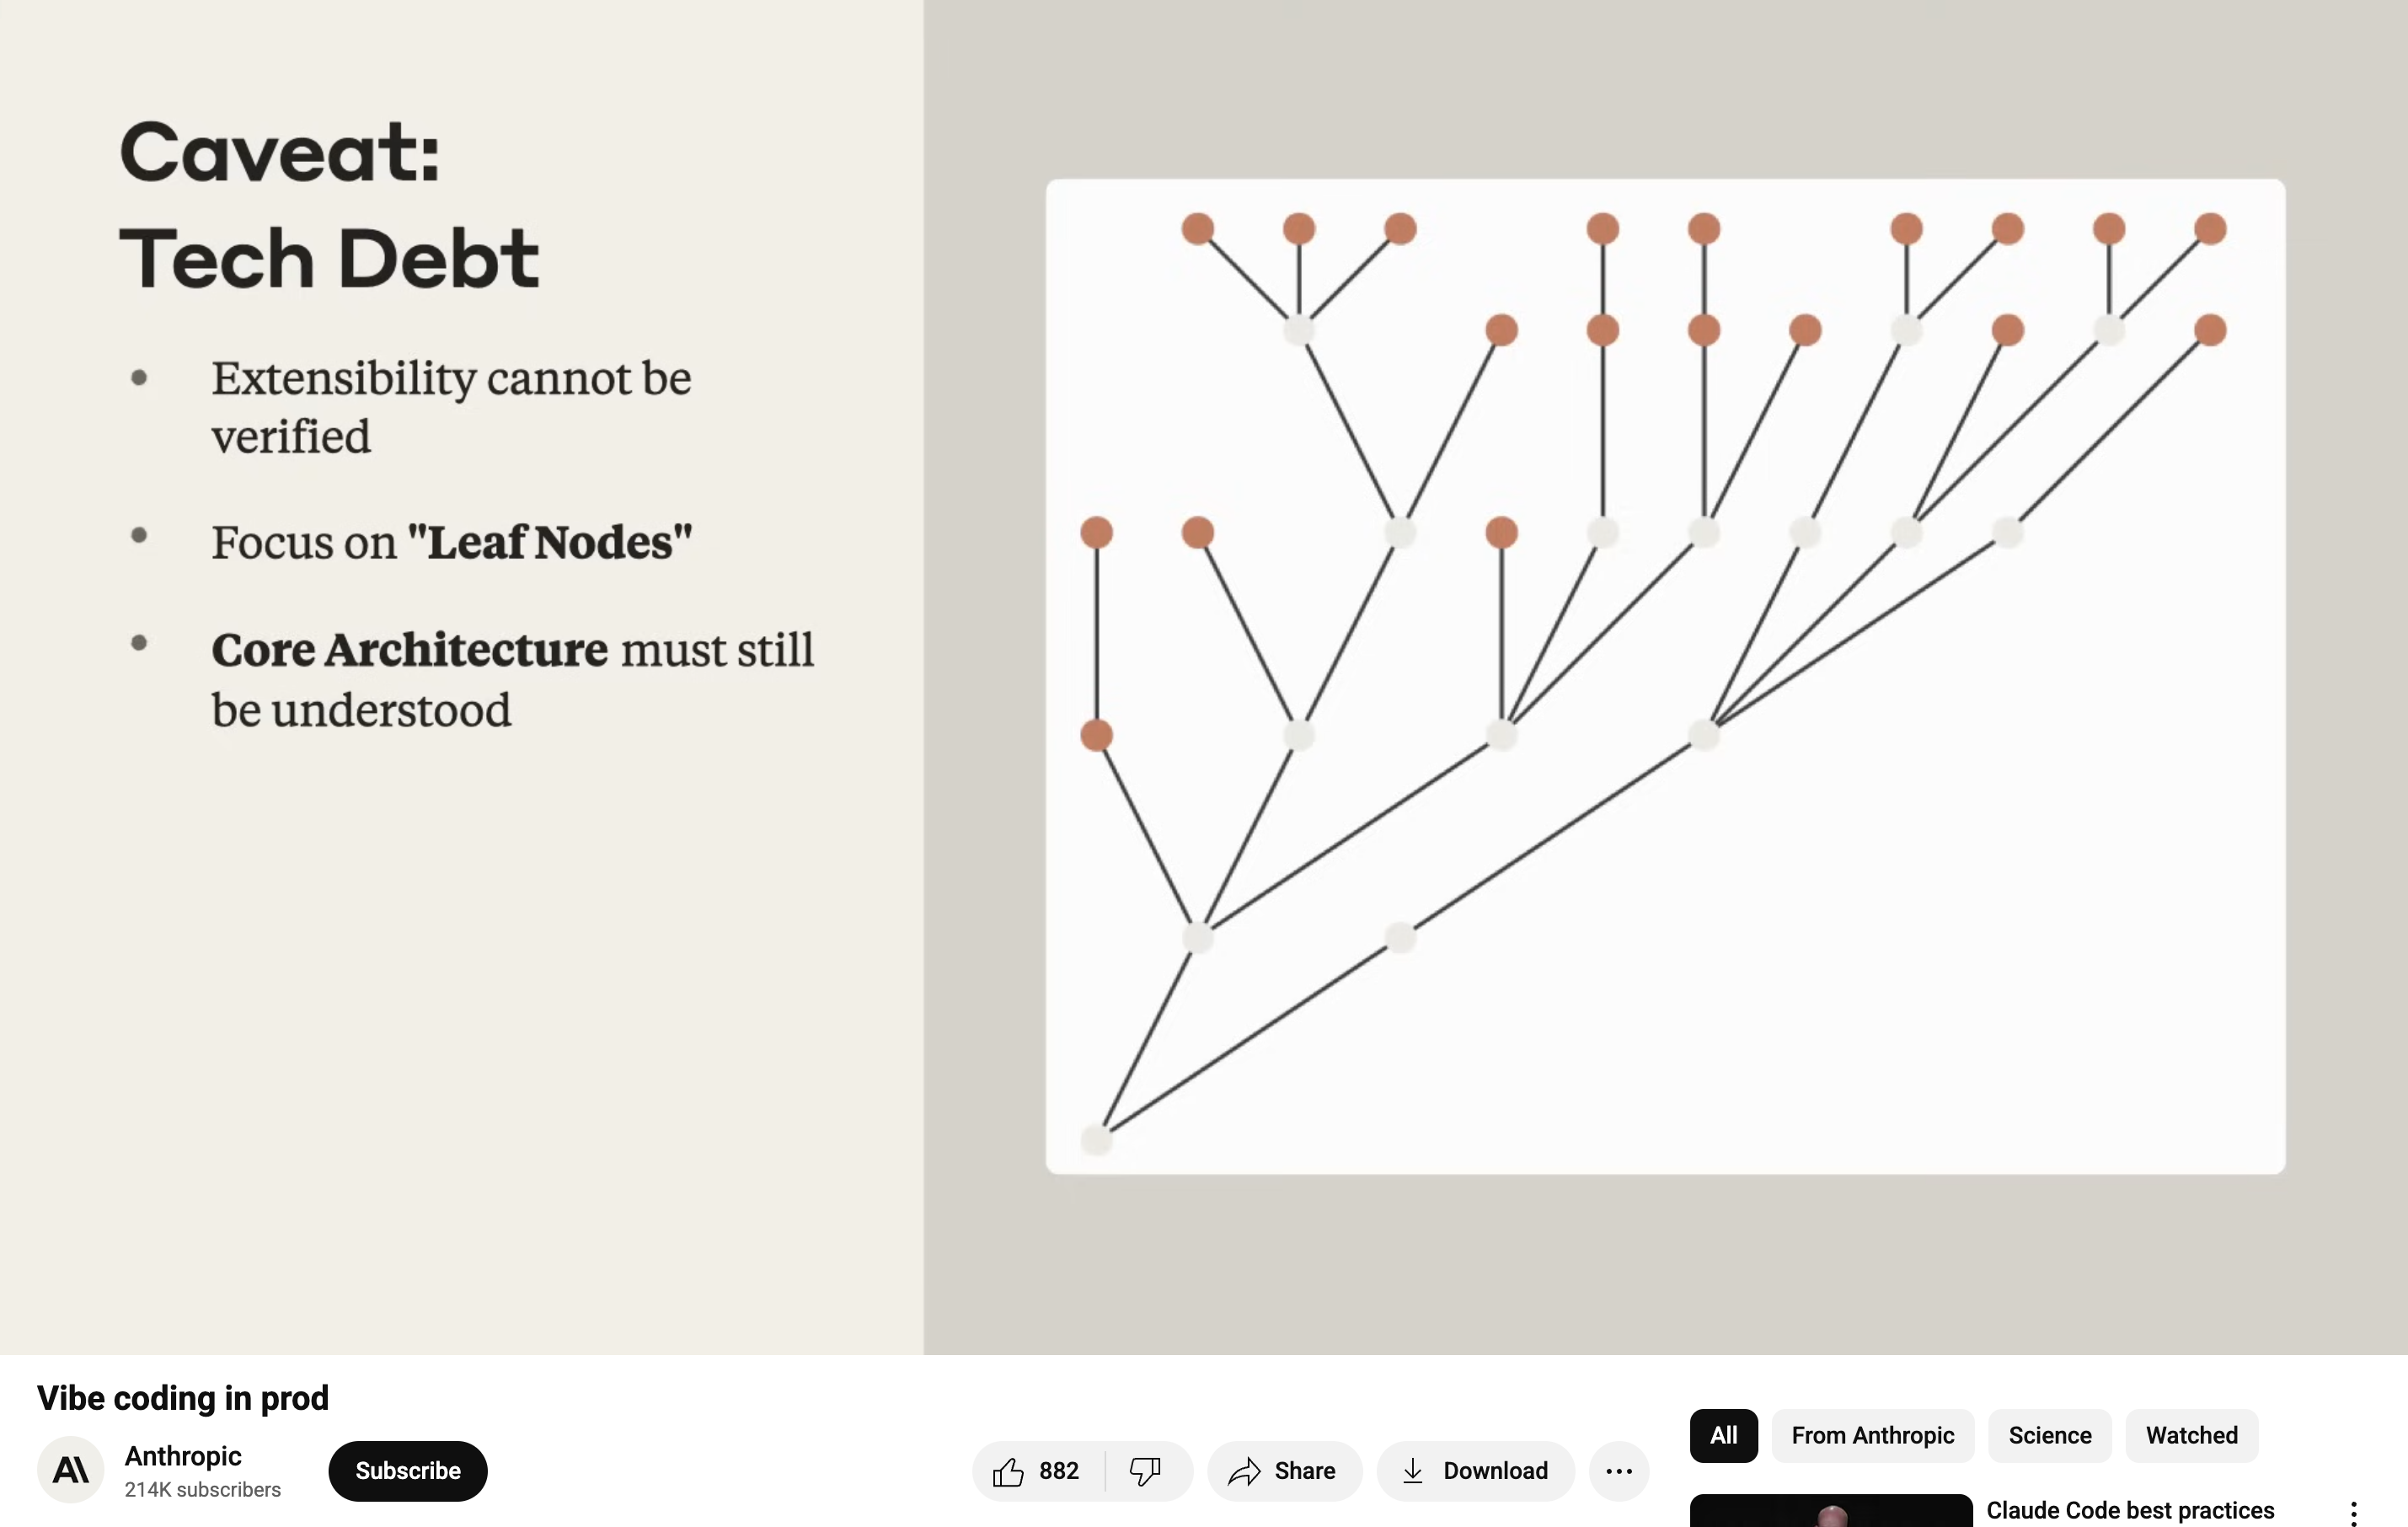
\includegraphics[keepaspectratio]{images/Anthropic Vibe Coding - Tech Debt Caveat.png}}\end{minipage}%

\end{figure}%

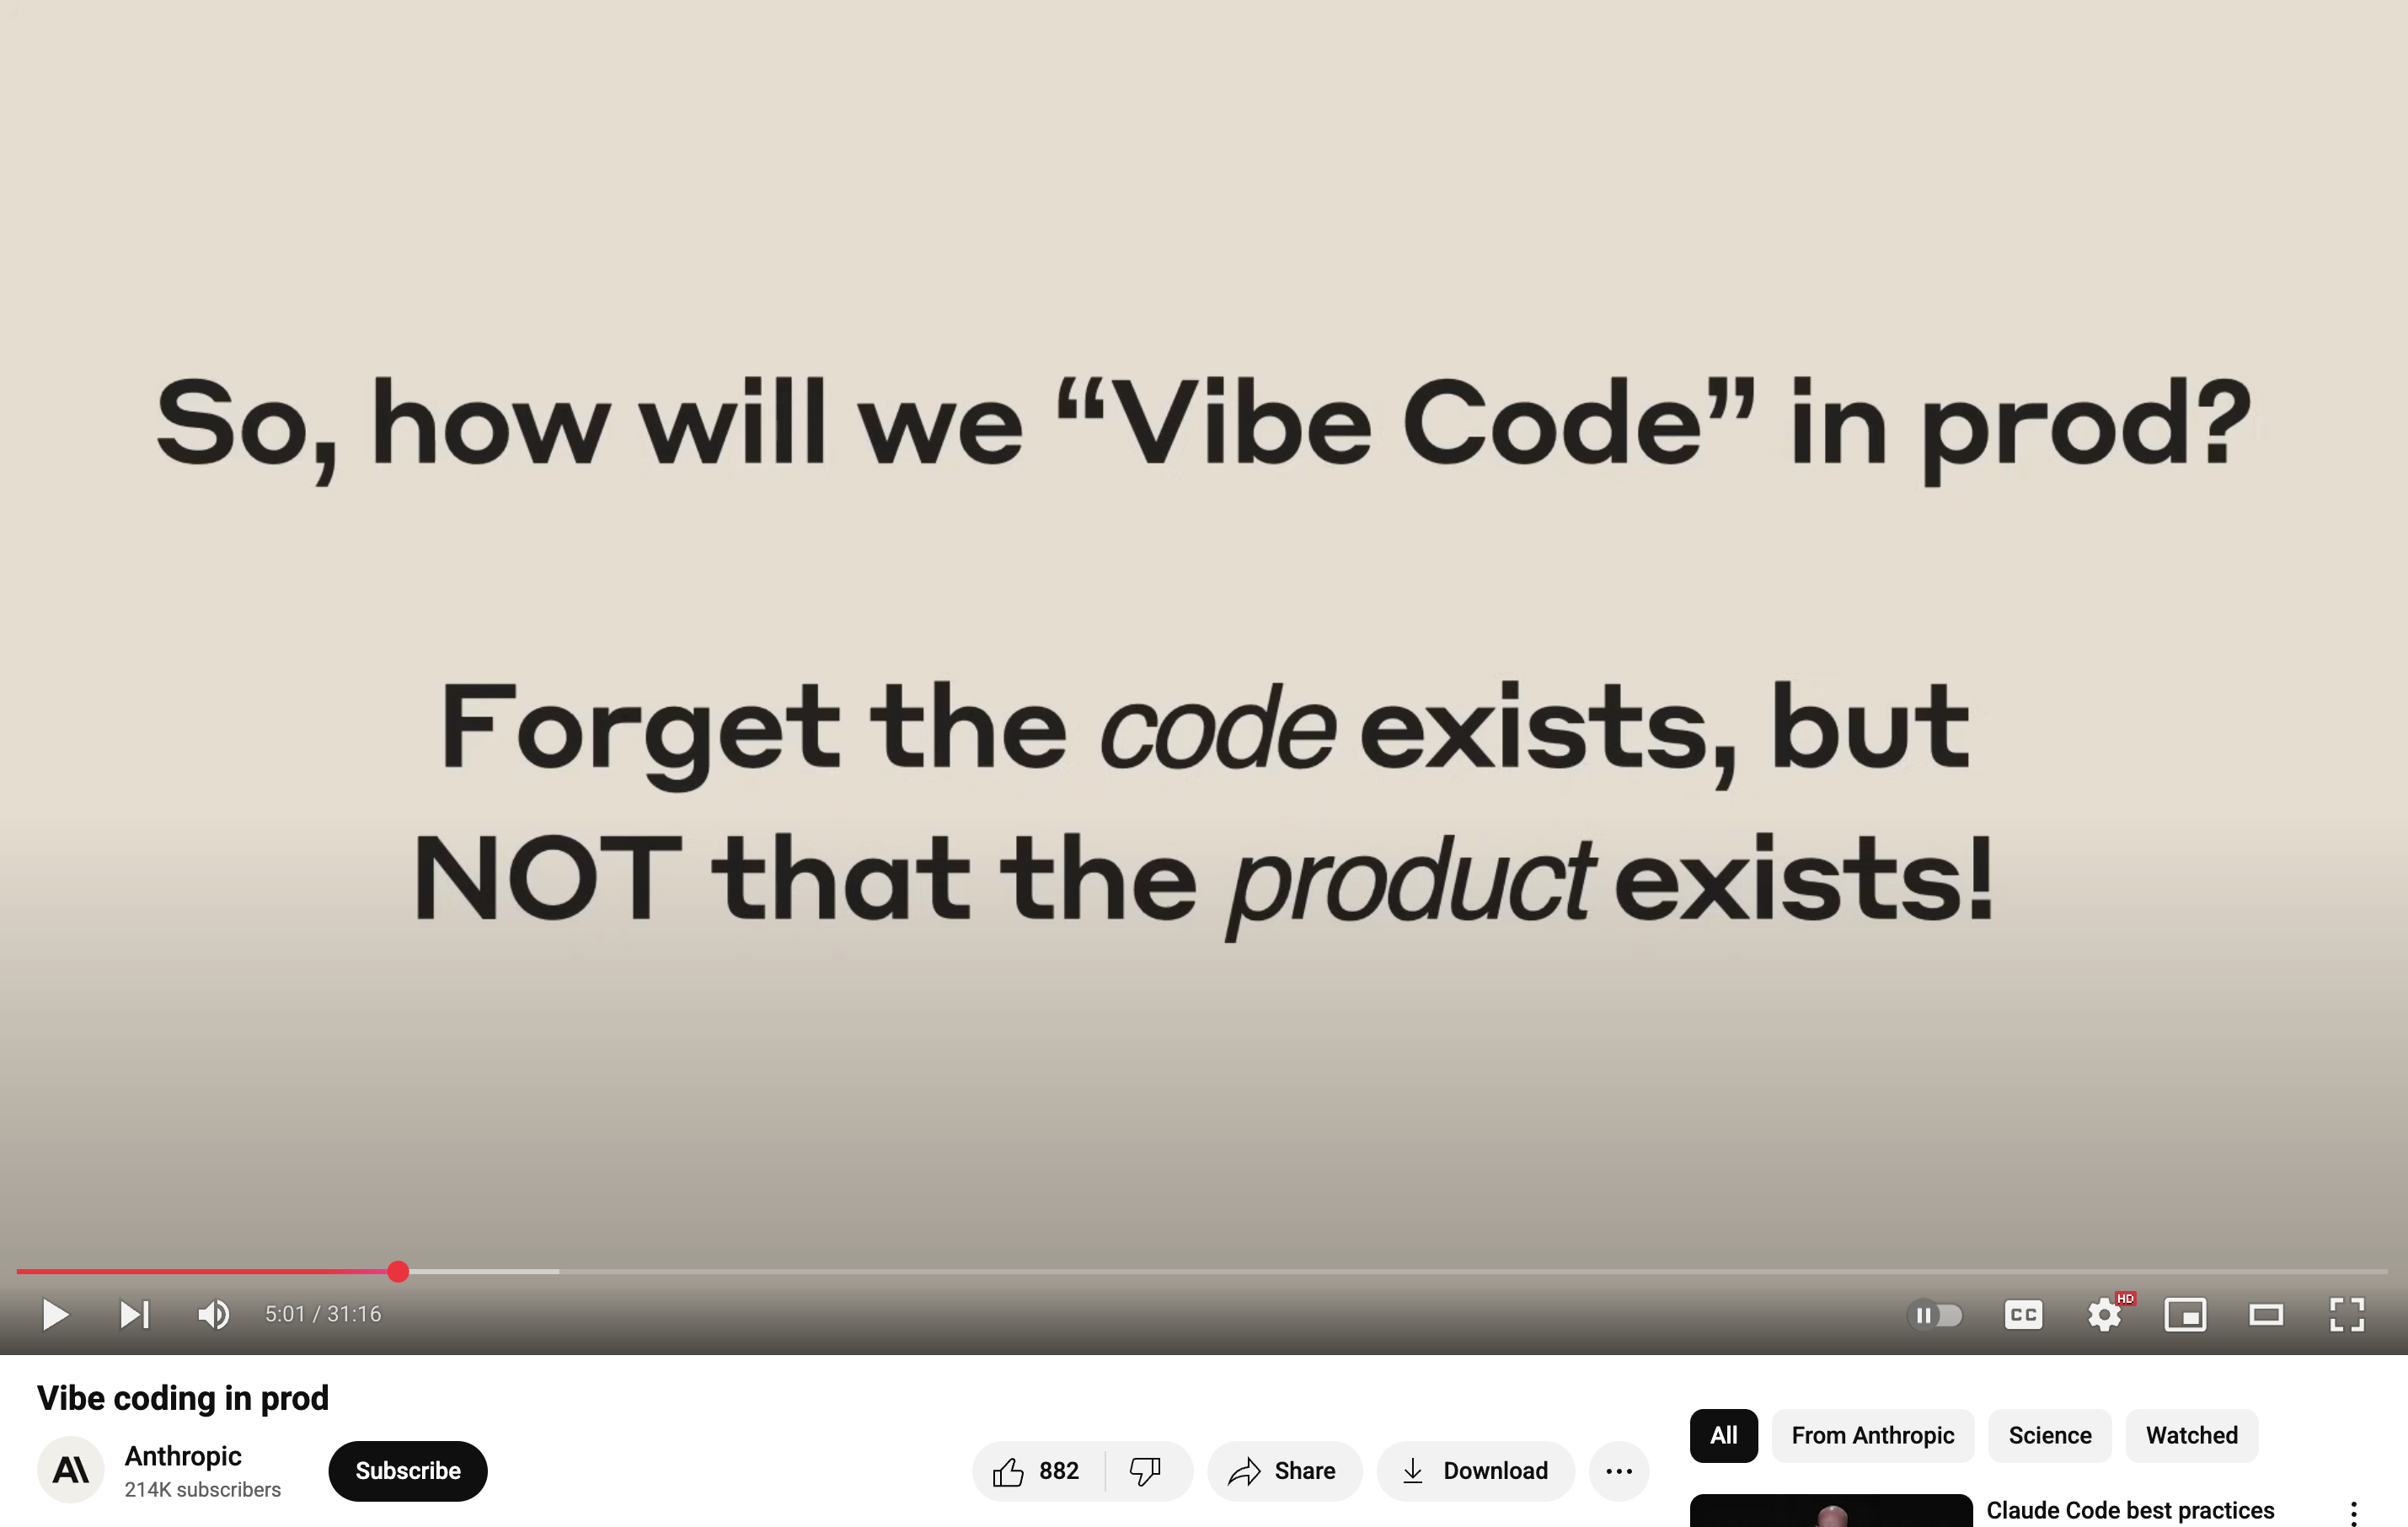
\includegraphics[width=0.5\linewidth,height=\textheight,keepaspectratio]{images/Anthropic Vibe Coding in Prod.png}

\textbf{I'm not qualified to talk about this.} Go to Anthropic's YouTube
page.
\end{frame}

\begin{frame}{\textbf{What This Talk IS About: The System for
High-Fidelity AI Partnership }}
\phantomsection\label{what-this-talk-is-about-the-system-for-high-fidelity-ai-partnership}
\textbf{Today, we're architecting a system that transforms digital chaos
into strategic advantage. I will introduce my 4-Stage Context
Engineering Pipeline---a methodology to turn your scattered thoughts,
emails, and documents into deterministic, high-value context for AI
collaboration.}

\textbf{The Transformation Journey:}

\begin{itemize}
\tightlist
\item
  \textbf{Stage 1:} Inception → Your thoughts become digital assets
\item
  \textbf{Stage 2:} Storage → Scattered data becomes deterministic
  context\\
\item
  \textbf{Stage 3:} Refinement → Raw information becomes actionable
  intelligence
\item
  \textbf{Stage 4:} Assembly → Perfect context orchestration for complex
  decisions
\end{itemize}

\textbf{Plus:} Examples showing these systems in action + AI's
deflationary impact

\textbf{My take:} AI is the great equalizer leaving only execution on
the table. If you're in this room, you're ahead of the curve.
\end{frame}

\begin{frame}
\end{frame}

\section{\texorpdfstring{\textbf{Session Ground
Rules}}{Session Ground Rules}}\label{session-ground-rules}

\begin{frame}{\textbf{Session Ground Rules}}
\begin{enumerate}
\tightlist
\item
  \textbf{Raise your hands!} Your contributions matter more than my
  content
\item
  \textbf{Clarify and Correct:} Share your stories and experiences
\item
  \textbf{This is a discussion} --- jump in via chat or hand raise
\end{enumerate}
\end{frame}

\begin{frame}
\end{frame}

\section{\texorpdfstring{\textbf{About Me}}{About Me}}\label{about-me}

\begin{frame}{\textbf{About Me}}
\textbf{Mo Battah} \textbar{} Recently VP, DevOps Engineering at Actabl

\textbf{Since leaving last month:}

\begin{itemize}
\tightlist
\item
  Advised on \textbf{\$10M+ in VC + PE transactions} across 2 deals
\item
  \textbf{Currently helping founders} in AI agents, cybersecurity, and
  defense tech
\item
  \textbf{These systems were the operational backbone} that enabled
  instant, high-fidelity context for due diligence and strategic
  analysis
\end{itemize}

\textbf{Active in Venture Capital:}

\begin{itemize}
\tightlist
\item
  Capital efficiency is in vogue, no `vibe coding' but tons of
  Cursor/Claude Code
\item
  \textbf{Portfolio:} ProtectAI, Dreadnode, Resourcely, Kodiak Robotics,
  Skydio
\end{itemize}

\textbf{Why this matters:} \emph{I use these systems daily to drive
business outcomes and operational efficiency.}
\end{frame}

\begin{frame}
\end{frame}

\section{\texorpdfstring{\textbf{Quick Poll: AI Tool
Experience}}{Quick Poll: AI Tool Experience}}\label{quick-poll-ai-tool-experience}

\begin{frame}{\textbf{Quick Poll: AI Tool Experience}}
\textbf{Show of hands to gauge experience levels:}

\begin{enumerate}
\item
  \textbf{Who has used Cursor / Windsurf?} \emph{(AI IDEs)}
\item
  \textbf{Who has used Claude Code?} \emph{(AI CLI)}
\item
  \textbf{Who has used Warp's agentic features?} \emph{(Agentic Dev
  Env)}
\item
  \textbf{Anyone tried Roo or Cline?} \emph{(FOSS Cursor)}
\item
  \textbf{Who here has worked with LaTeX for document or report
  generation?} \emph{(Gold-standard typesetting)}
\end{enumerate}

\emph{This helps me calibrate how deep to go on technical details
vs.~practical applications}
\end{frame}

\begin{frame}
\end{frame}

\section{\texorpdfstring{\textbf{The Ladder of
Abstraction}}{The Ladder of Abstraction}}\label{the-ladder-of-abstraction}

\begin{frame}{\textbf{From Prompting to Partnership}}
\phantomsection\label{from-prompting-to-partnership}
\textbf{Most people are at Level 1. Some might be at Level 2. My
favorite is Level 3.}

\textbf{Level 1: Conversational AI} - ChatGPT, Claude, Gemini as
baseline assistants

\textbf{Level 2: Integrated Assistants (IDE Extensions)}\\
- Cursor, Windsurf, Roo - they read codebases, propose plans, modify
code with approval

\textbf{Level 3: Agentic Partners (CLI Tools)} - Claude Code, Gemini CLI
- operate within terminal, execute scripts, manage files
\end{frame}

\begin{frame}
\end{frame}

\section{\texorpdfstring{\textbf{The Token Economy
Reality}}{The Token Economy Reality}}\label{the-token-economy-reality}

\begin{frame}{\textbf{Google's Explosive Growth in AI Usage}}
\phantomsection\label{googles-explosive-growth-in-ai-usage}
\begin{figure}[H]

{\centering 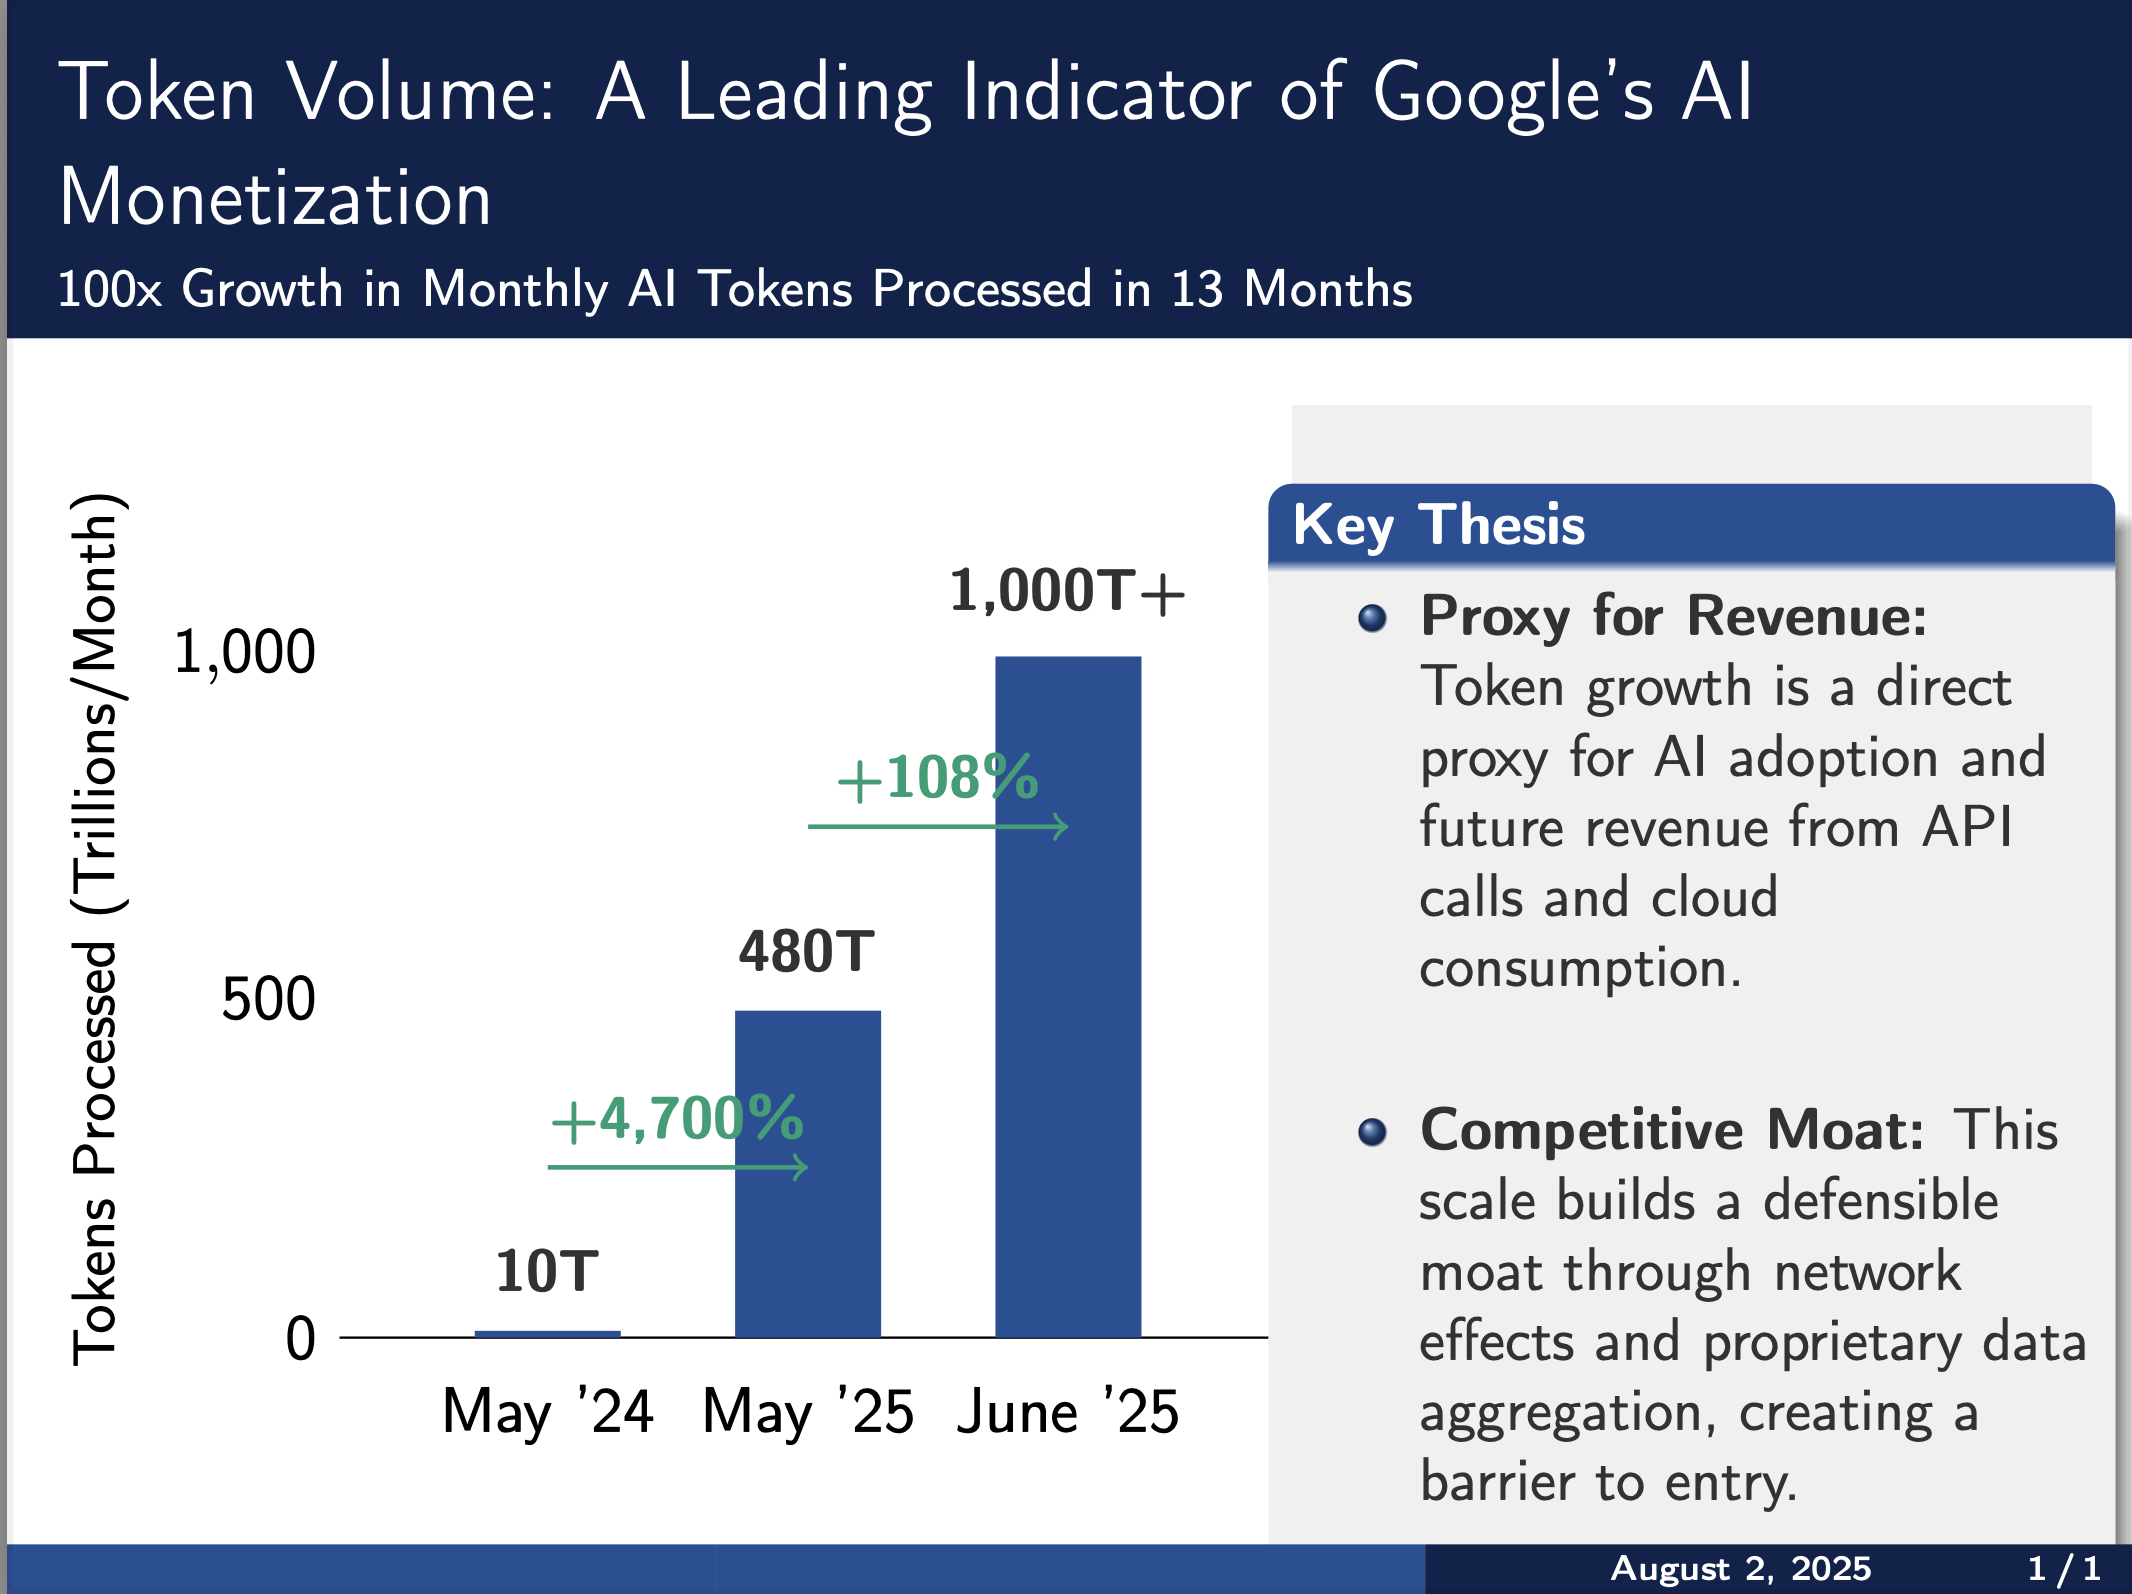
\includegraphics[width=0.9\linewidth,height=\textheight,keepaspectratio]{images/One Quadrillion Tokens Growth Chart.png}

}

\caption{Growth chart showing exponential increase}

\end{figure}%
\end{frame}

\begin{frame}{\textbf{What This Means}}
\phantomsection\label{what-this-means}
The world is rapidly transforming into \textbf{a world of tokens} ---
where these tokens have equivalency to human thought.

\textbf{My approach:} Replace my ``negligible-value thoughts'' with AI
tokens wherever possible.

\textbf{Examples of negligible-value thinking:} - The 30 minutes spent
manually collating stakeholder feedback from three different email
threads before a planning meeting - The mental context-switching
required to parse a dozen downloaded reports, PDFs, and logs to
synthesize a single coherent summary\\
- Routine analysis tasks that take me hours but AI handles instantly

\textbf{The Goal:} Use AI as a thought partner, gut check, and
improvement tool --- freeing my brain for high-value decisions
\end{frame}

\begin{frame}
\end{frame}

\section{\texorpdfstring{\textbf{So How Do You Actually Do
This?}}{So How Do You Actually Do This?}}\label{so-how-do-you-actually-do-this}

\begin{frame}{\textbf{So How Do You Actually Do This?}}
\textbf{The challenge:} You can't just throw problems at AI and expect
it to replace your thinking effectively.

\textbf{You need a systematic approach} to ensure AI has the same
contextual knowledge you would have when making decisions.

\textbf{Enter: Context Engineering} --- the 4-stage system that makes
token replacement actually work.
\end{frame}

\begin{frame}
\end{frame}

\section{\texorpdfstring{\textbf{Context Engineering: The
Foundation}}{Context Engineering: The Foundation}}\label{context-engineering-the-foundation}

\begin{frame}{\textbf{Context Engineering: The Foundation}}
\begin{quote}
\emph{``Context is everything, yet context is what's missing.''}
\end{quote}

\textbf{Context is gold. Without good context engineering, prompt
engineering is irrelevant.}

\textbf{Bad context doesn't just give you bad outputs; it poisons your
entire decision-making process.}

\textbf{Context engineering is the foundation of all effective AI use.}
\end{frame}

\begin{frame}
\end{frame}

\section{\texorpdfstring{\textbf{The 4-Stage Context Engineering
Pipeline}}{The 4-Stage Context Engineering Pipeline}}\label{the-4-stage-context-engineering-pipeline}

\begin{frame}{\textbf{The 4-Stage Context Engineering Pipeline}}
\textbf{The system for manufacturing perfect, context-rich prompts}

\begin{enumerate}
\tightlist
\item
  \textbf{Inception} → Capture high-bandwidth thought as structured
  digital assets
\item
  \textbf{Storage} → Engineer a deterministic context repository, your
  ``second brain''\\
\item
  \textbf{Refinement} → Synthesize raw data into actionable, strategic
  intelligence
\item
  \textbf{Assembly} → Orchestrate massive, holistic prompts for
  insurmountable leverage
\end{enumerate}

\textbf{This pipeline ensures AI has the same contextual knowledge I
would have when making decisions --- often better, because it can
cross-reference everything instantly.}
\end{frame}

\begin{frame}{\textbf{Stage 1: Context Inception}}
\phantomsection\label{stage-1-context-inception}
\begin{block}{\textbf{Wispr Flow --- High-Bandwidth Thought Capture}}
\phantomsection\label{wispr-flow-high-bandwidth-thought-capture}
\begin{itemize}
\tightlist
\item
  \textbf{\textasciitilde100K words/month} voice dictation
\item
  \textbf{Keyboards are the bottleneck} to thought capture
\item
  Real-time verbal brainstorming → structured AI-ready text
\item
  Applications range from email composition to complex architecture
  problems
\end{itemize}

\textbf{Key Insight:} Your thoughts become digital assets

\begin{figure}[H]

{\centering 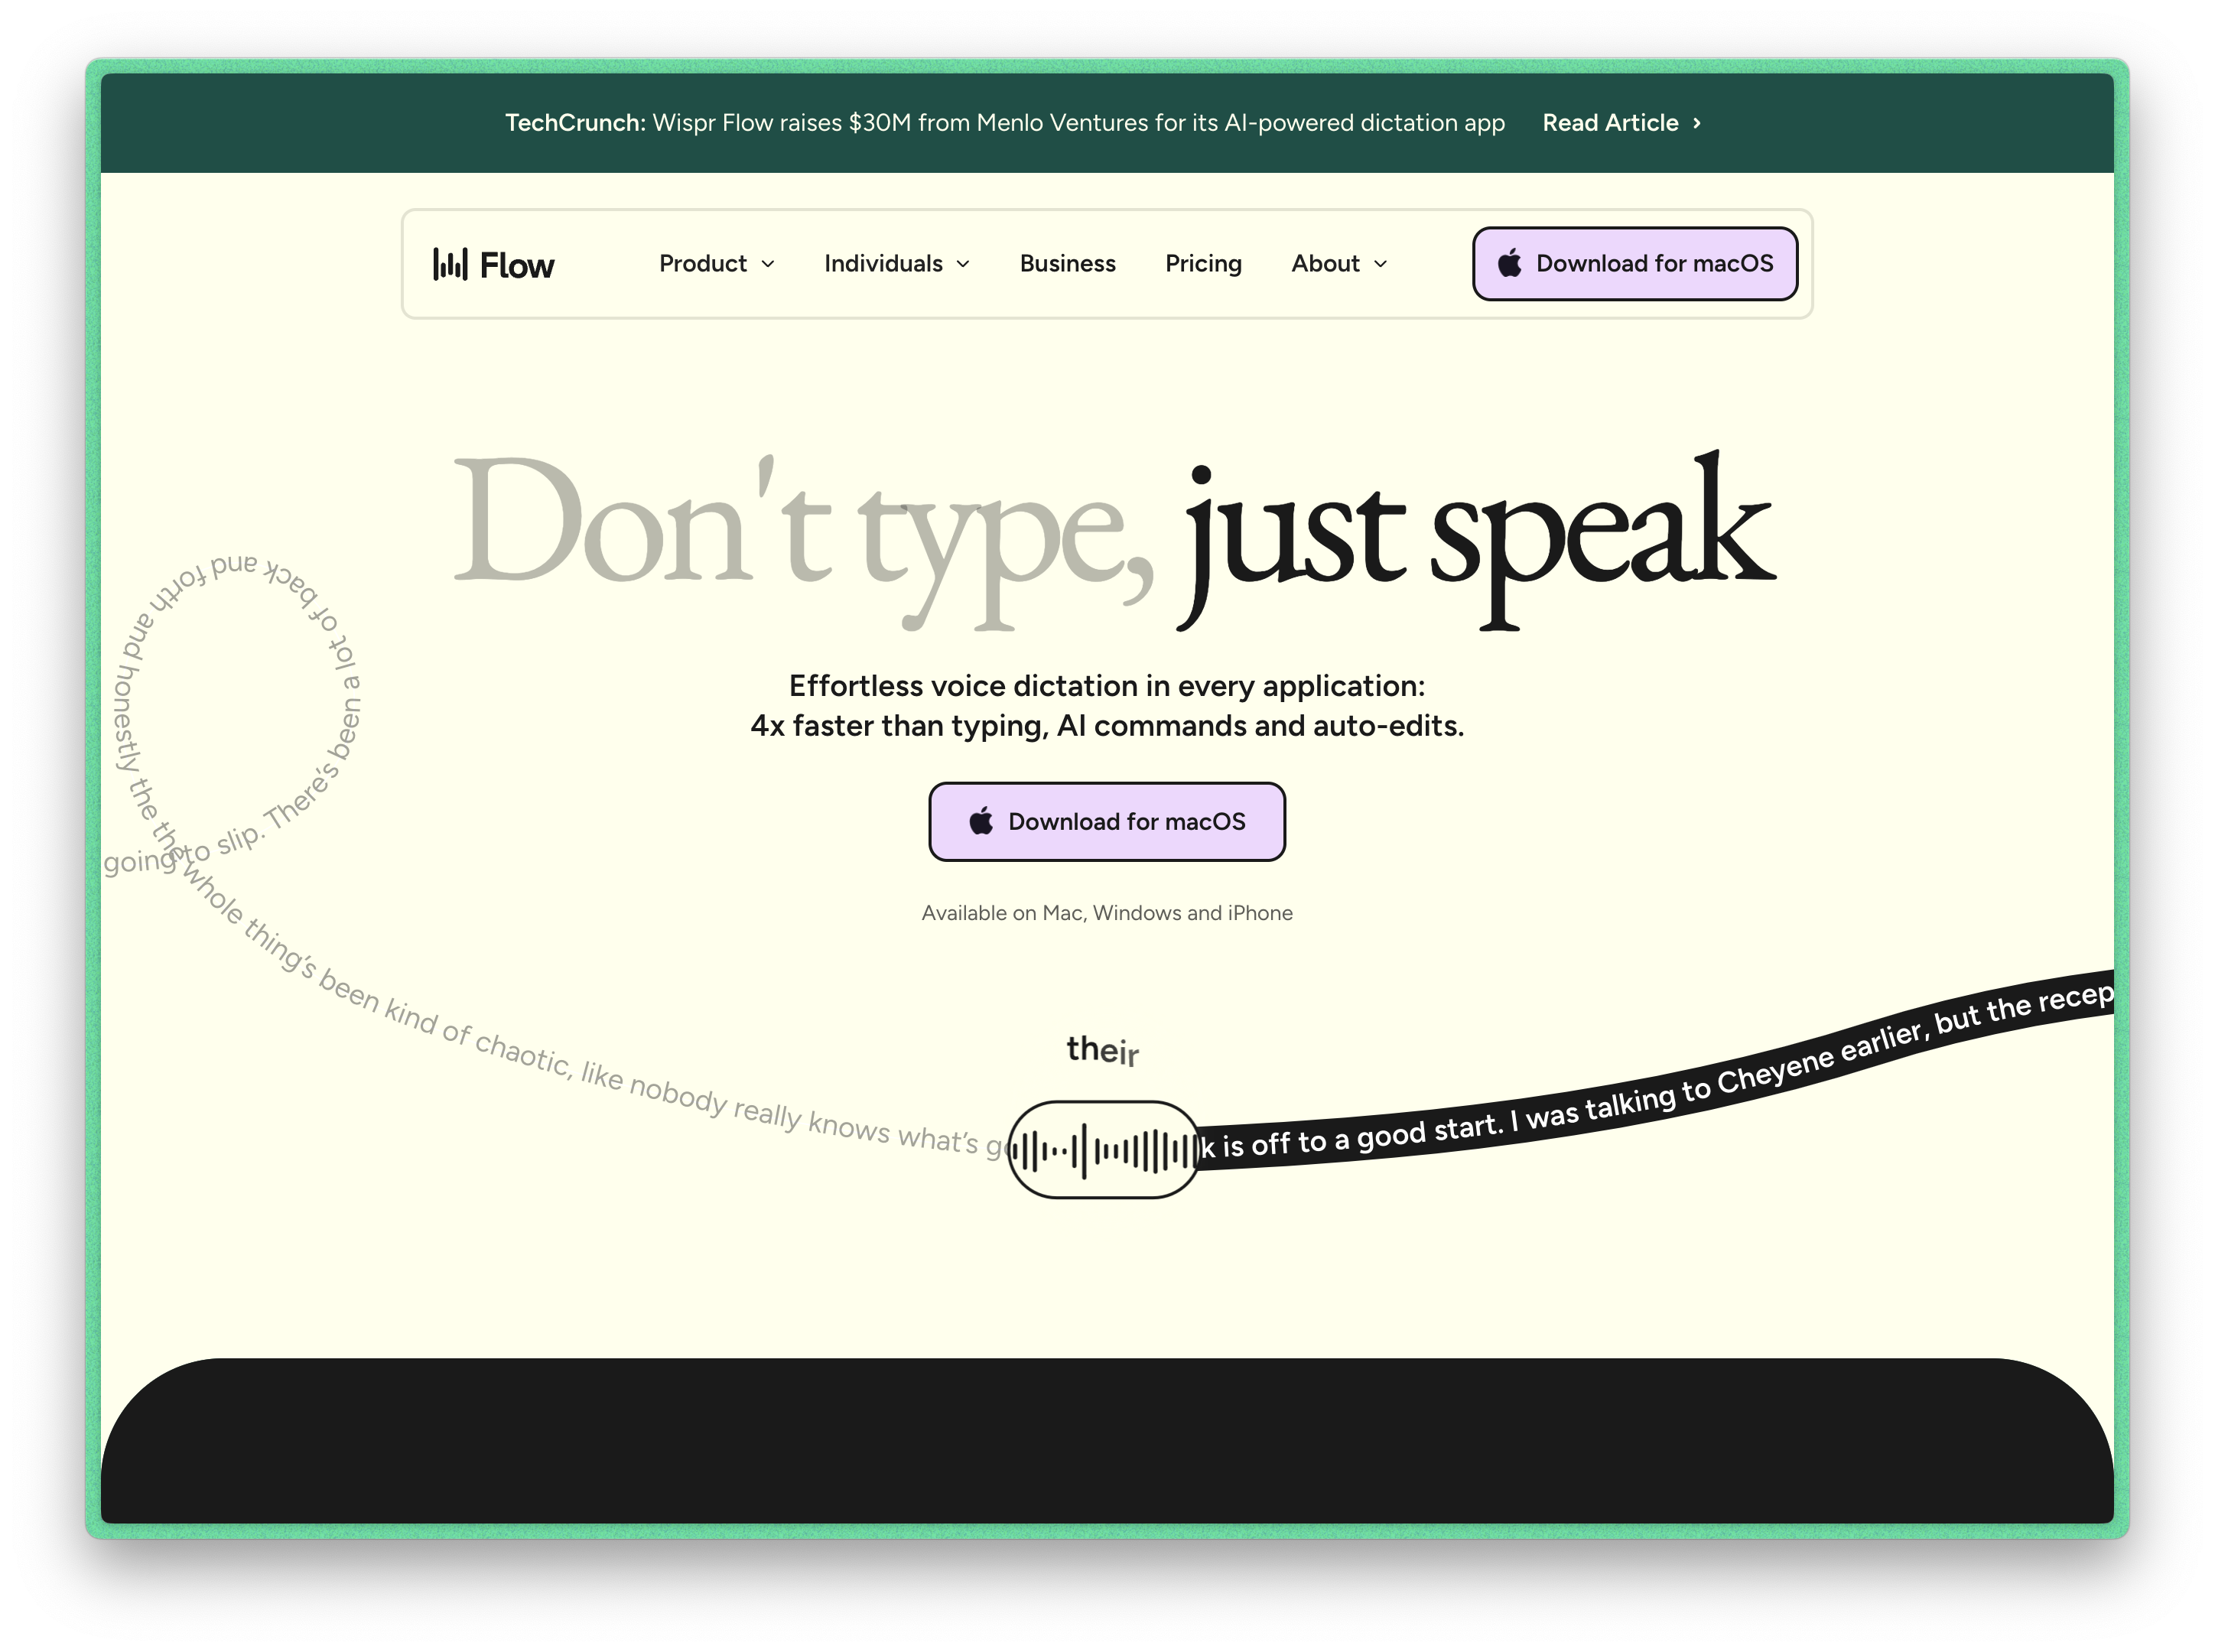
\includegraphics[width=0.75\linewidth,height=\textheight,keepaspectratio]{images/wisprflow.png}

}

\caption{Wispr Flow - Work at the speed you think in every application}

\end{figure}%
\end{block}
\end{frame}

\begin{frame}{\textbf{Stage 2: Context Storage \& Management}}
\phantomsection\label{stage-2-context-storage-management}
\begin{block}{\textbf{All Context Sources → Git as Markdown}}
\phantomsection\label{all-context-sources-git-as-markdown}
\textbf{All Context Sources → Markdown Files:}

\begin{itemize}
\tightlist
\item
  \textbf{Wispr Flow transcripts} from Stage 1 → Stored permanently
\item
  \textbf{Call transcriptions} via Google AI Studio (free)
\item
  \textbf{Email archives} downloaded → AI flattened → Git
\item
  \textbf{Strategic thinking} → Career goals, brand guidelines, decision
  frameworks
\item
  \textbf{Technical contexts} → Architecture challenges, project
  requirements
\item
  \textbf{Documents \& artifacts} → Reports, PDFs, SOWs, contracts
  (converted to Markdown)
\end{itemize}

\textbf{Why Not MCP Servers:}

\begin{itemize}
\tightlist
\item
  Probabilistic outcomes, unreliable retrieval
\item
  \textbf{Solution:} Pre-processed, verified context files
\end{itemize}
\end{block}
\end{frame}

\begin{frame}
\begin{block}{\textbf{Context in Action: SOW Example}}
\phantomsection\label{context-in-action-sow-example}
\emph{Statement of Work + emails + call transcripts = complete project
context}

\textbf{AI Query:} \emph{``Based on our SOW, emails, and call
transcripts, where are we on this project? If the vendor is behind, what
are our negotiation options?''}

\textbf{Result:} Instant situational awareness and strategic options
\end{block}
\end{frame}

\begin{frame}
\emph{⚠️ Security Note: Use private repos, strong permissions, and avoid
committing overly personal PII or confidential business information}
\end{frame}

\begin{frame}
\begin{block}{\textbf{Example Repository Structure}}
\phantomsection\label{example-repository-structure}
\begin{columns}[T]
\begin{column}{0.5\linewidth}
\textbf{📁 Technical Decisions} - Architecture reviews - Incident
postmortems\\
- Tech debt assessments

\textbf{👥 Team Management} - Hiring \& interviews - Performance reviews
- One-on-one contexts
\end{column}

\begin{column}{0.5\linewidth}
\textbf{🤝 Vendor Relationships} - Contract negotiations - Tool
evaluations - Procurement decisions

\textbf{🎯 Strategic Planning} - Quarterly roadmaps - Budget planning -
Investment decisions
\end{column}
\end{columns}

\textbf{Key Benefits:} Deterministic • AI-native • Version controlled
\end{block}
\end{frame}

\begin{frame}{\textbf{Stage 3: Context Enrichment \& Refinement}}
\phantomsection\label{stage-3-context-enrichment-refinement}
\begin{block}{\textbf{From Scattered Assets to Strategic Intelligence}}
\phantomsection\label{from-scattered-assets-to-strategic-intelligence}
\begin{columns}[T]
\begin{column}{0.45\linewidth}
\textbf{BEFORE: Raw Assets}

\begin{itemize}
\tightlist
\item
  📝 Voice note about issue\\
\item
  📧 Email thread with stakeholders\\
\item
  🎫 Jira tickets on the problem\\
\item
  📞 Call transcript discussing solutions
\end{itemize}

\emph{Scattered, disconnected, requiring manual synthesis}
\end{column}

\begin{column}{0.1\linewidth}
\textbf{AI}\\
\textbf{Synthesis}\\
\textbf{→}
\end{column}

\begin{column}{0.45\linewidth}
\textbf{AFTER: Enriched Context}

\textbf{📋 Comprehensive Problem Context}

\begin{itemize}
\tightlist
\item
  All stakeholder positions identified
\item
  Solution options consolidated\\
\item
  Risk factors highlighted
\item
  Strategic recommendations ready
\end{itemize}

\emph{Single authoritative source of truth}
\end{column}
\end{columns}

\textbf{Real Example:} \emph{Engineering problem voice note + team call
transcript + Jira tickets → comprehensive problem context with all
stakeholder views and solution options}

\textbf{This transforms AI from a search tool into a strategic advisor.}
\end{block}
\end{frame}

\begin{frame}{\textbf{Stage 4: Context Assembly \& Orchestration}}
\phantomsection\label{stage-4-context-assembly-orchestration}
\begin{block}{\textbf{Prompt Tower --- The Ultimate Context Assembler}}
\phantomsection\label{prompt-tower-the-ultimate-context-assembler}
\textbf{VSCode Extension Features:}

\begin{itemize}
\tightlist
\item
  Select files: transcripts, emails, reports, context files
\item
  Custom prompt prefixes/suffixes
\item
  \textbf{Massive context windows} (\textgreater100K tokens)
\item
  One-click → clipboard → Gemini
\end{itemize}

\textbf{Daily Use Cases:}

\begin{itemize}
\tightlist
\item
  Pre-call prep with full conversation history
\item
  Strategic analysis with complete relationship context
\item
  Engineering problems with codebase + team discussions
\end{itemize}
\end{block}
\end{frame}

\begin{frame}[fragile]{\textbf{Examples: Engineering Principles
Applied}}
\phantomsection\label{examples-engineering-principles-applied}
\begin{block}{\textbf{AI-Assisted Technical Analysis: Automating the
Last Mile}}
\phantomsection\label{ai-assisted-technical-analysis-automating-the-last-mile}
\begin{itemize}
\tightlist
\item
  AI content + LaTeX precision
\item
  Programmatic TikZ diagrams
\item
  \texttt{quarto\ render} → Professional PDF
\end{itemize}
\end{block}
\end{frame}

\begin{frame}
\begin{block}{\textbf{The AI-Powered Feedback Loop: Systematizing
Self-Improvement}}
\phantomsection\label{the-ai-powered-feedback-loop-systematizing-self-improvement}
\begin{itemize}
\tightlist
\item
  Record calls → AI analysis
\item
  Communication gap identification
\item
  Negotiation improvement tracking
\end{itemize}
\end{block}
\end{frame}

\begin{frame}
\begin{block}{\textbf{The AI Vocabulary Coach: Extending Finite
Expertise Infinitely}}
\phantomsection\label{the-ai-vocabulary-coach-extending-finite-expertise-infinitely}
\begin{itemize}
\tightlist
\item
  Norman Lewis + Tom Heehler principles
\item
  Call transcript analysis
\item
  Vocabulary edge expansion
\end{itemize}
\end{block}
\end{frame}

\begin{frame}
\begin{block}{\textbf{Automated CRM Enrichment: Systematizing
Serendipity}}
\phantomsection\label{automated-crm-enrichment-systematizing-serendipity}
\begin{itemize}
\tightlist
\item
  Connection research + context matching (ex: fits your ideal customer
  profile)
\item
  Relationship mapping (ex: 3 connections at target customer, infers
  hierarchy)
\end{itemize}

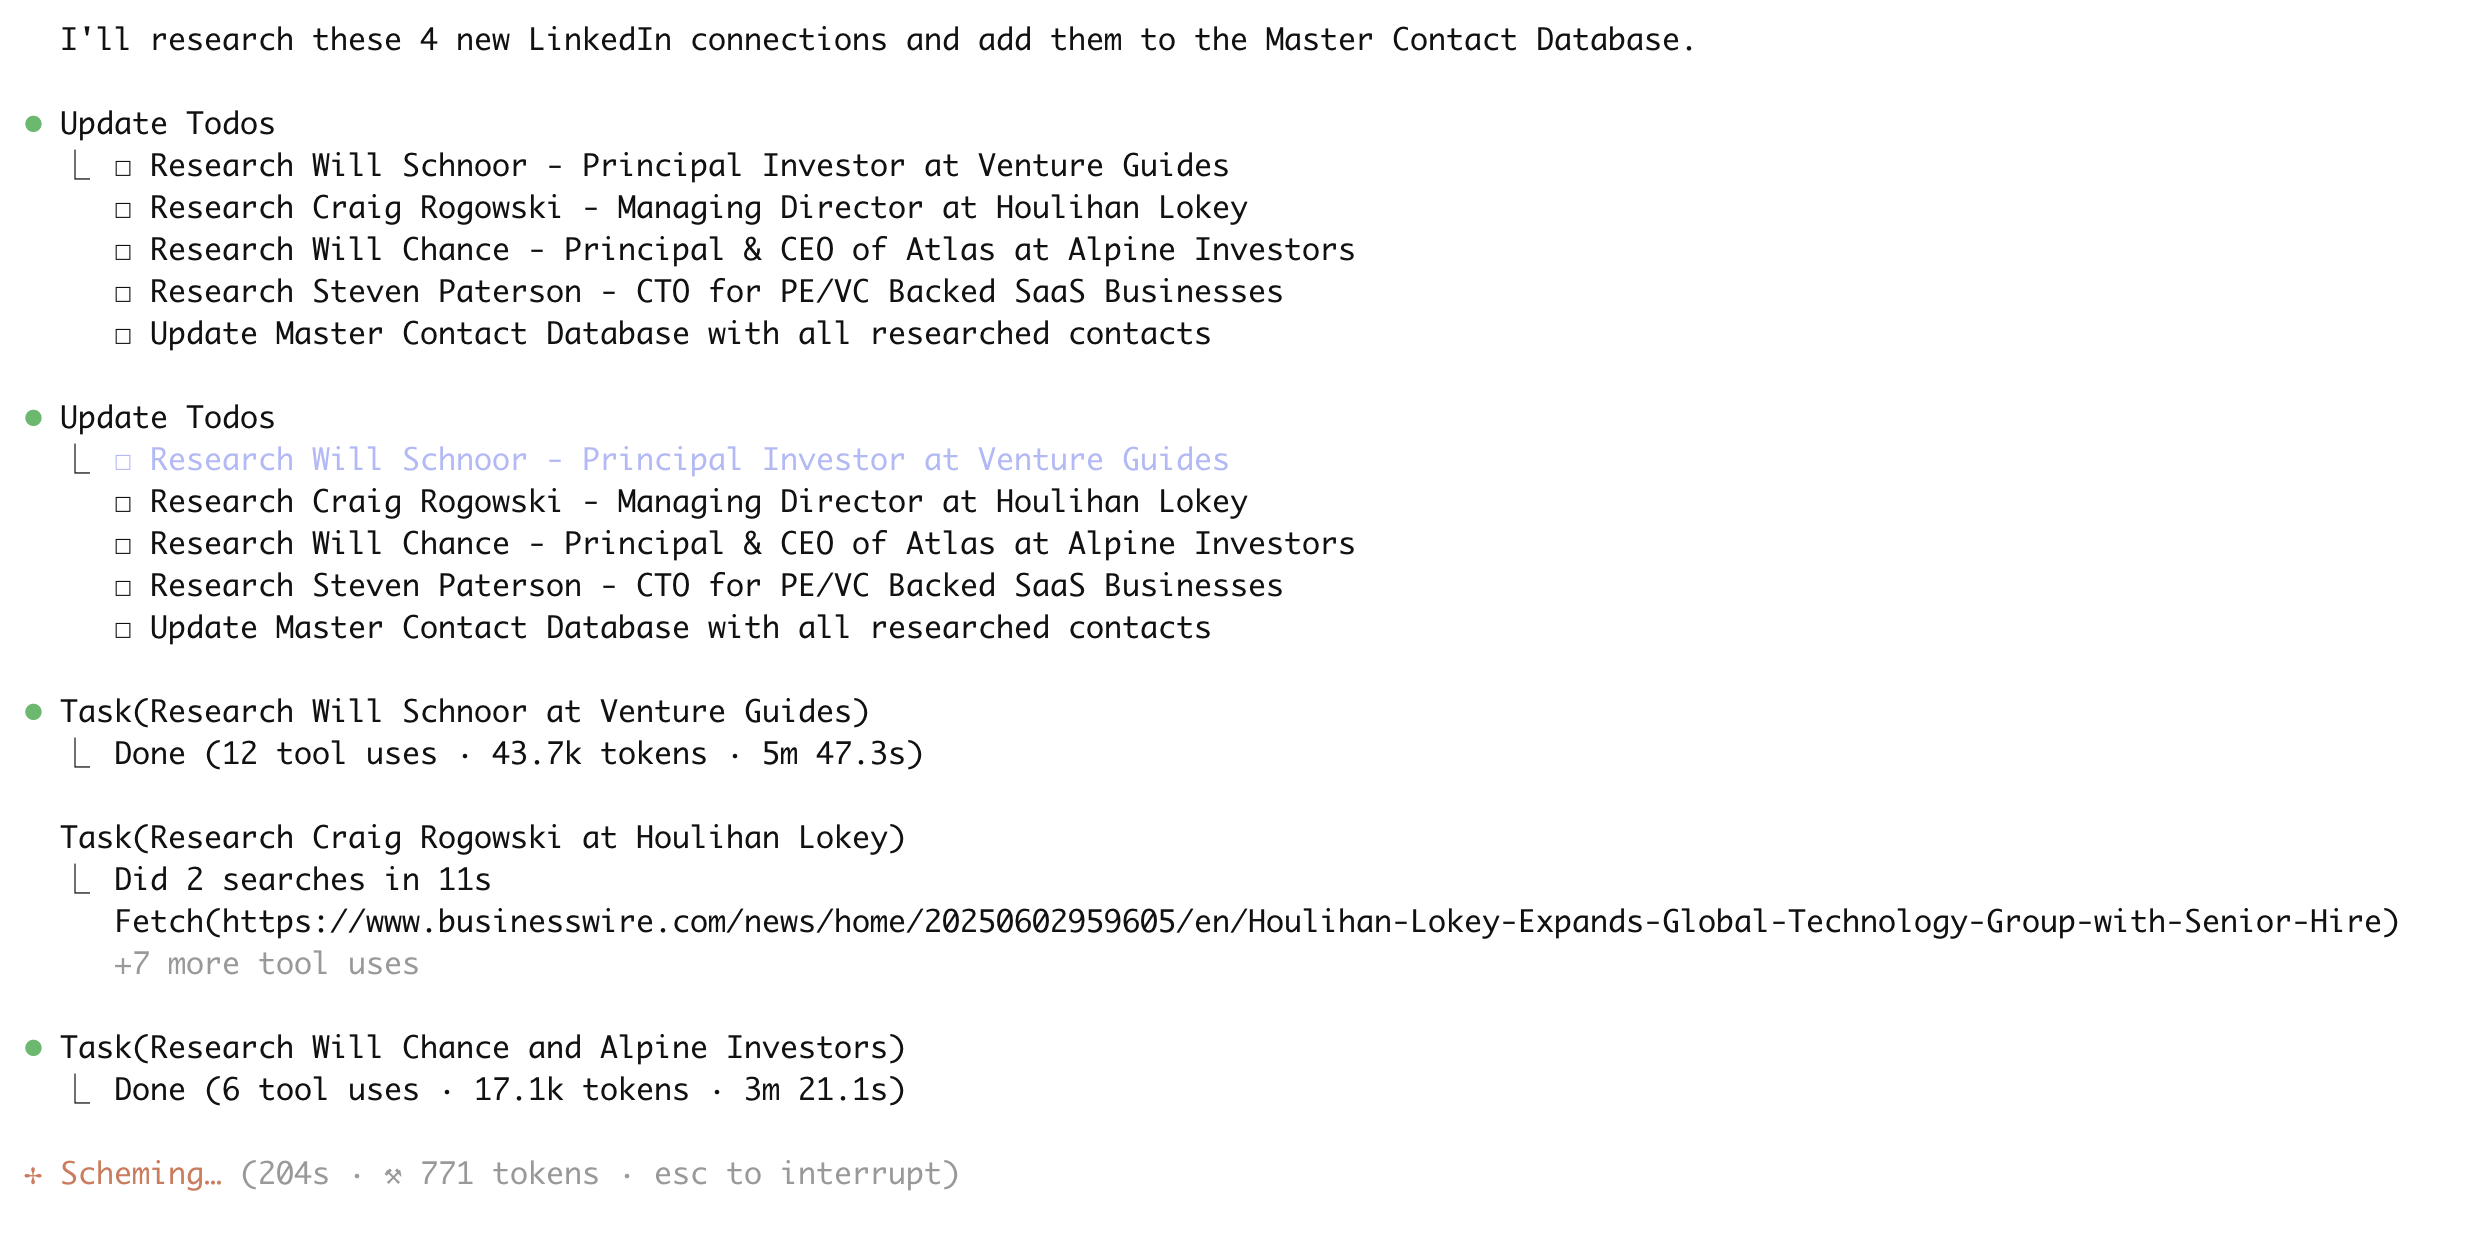
\includegraphics[width=0.9\linewidth,height=\textheight,keepaspectratio]{images/automatic-crm-via-linkedin-data.png}
\end{block}
\end{frame}

\begin{frame}
\begin{block}{\textbf{The Modular Resume System: A Case Study in
``Documentation as Code''}}
\phantomsection\label{the-modular-resume-system-a-case-study-in-documentation-as-code}
\begin{itemize}
\tightlist
\item
  Extensible LaTeX system
\item
  Source-of-truth data → Multiple formats
\item
  AI-powered customization (Amazon-specific in 10 minutes)
\end{itemize}
\end{block}
\end{frame}

\begin{frame}
\end{frame}

\section{\texorpdfstring{\textbf{The Bigger
Picture}}{The Bigger Picture}}\label{the-bigger-picture}

\begin{frame}{\textbf{AI as a Deflationary Force}}
\phantomsection\label{ai-as-a-deflationary-force}
\textbf{Reducing costs of critical services:}

\begin{itemize}
\tightlist
\item
  \textbf{Skydio}: Power line inspection → Reduced electricity costs
\item
  \textbf{Kodiak}: Autonomous trucking in Permian Basin → Lower oil
  costs
\item
  \textbf{Gecko Robotics}: Autonomous structural integrity robots →
  Lower maintenance, higher efficiency
\item
  \textbf{My systems}: Manual research/analysis → Automated intelligence
  gathering
\end{itemize}

\textbf{This is the real AI revolution:} Not replacing humans, but
making services drastically cheaper.
\end{frame}

\begin{frame}{\textbf{Personal → Professional Transformation}}
\phantomsection\label{personal-professional-transformation}
\textbf{These systems start personal, then naturally extend to work:}

\begin{itemize}
\tightlist
\item
  Context engineering for business relationships → client management
\item
  Voice capture for personal thoughts → meeting prep and follow-up
\item
  AI-assisted analysis for personal decisions → strategic business
  analysis
\end{itemize}

\textbf{The transition happens individually first, then
organizationally. You don't need permission to start building leverage.}
\end{frame}

\begin{frame}{\textbf{Case Study: AI-Powered Career Strategy}}
\phantomsection\label{case-study-ai-powered-career-strategy}
\textbf{The Odyssey Plan Exercise:} Feed your resume into Gemini and ask
for three career trajectories:

\begin{enumerate}
\tightlist
\item
  \textbf{Continue Current Path} - Natural progression
\item
  \textbf{Pivot Path} - Different direction using existing skills\\
\item
  \textbf{Wild Card Path} - Completely unexpected possibilities
\end{enumerate}

\textbf{My Generated Paths:} CTO, Operating Partner at PE fund, M\&A
Consultant, Venture Fund role, Entrepreneur in Residence

\textbf{The System in Action:} - \textbf{Strategic Context Files:}
Career paths + ``current career thinking'' - \textbf{Opportunity
Evaluation:} AI evaluates new opportunities against your context

\textbf{Result:} Like having a career coach who's thought 5-10 years
ahead with high-fidelity scenarios.
\end{frame}

\begin{frame}
\end{frame}

\section{\texorpdfstring{\textbf{Conclusion \&
Discussion}}{Conclusion \& Discussion}}\label{conclusion-discussion}

\begin{frame}{\textbf{Why This Matters}}
\phantomsection\label{why-this-matters}
\textbf{These aren't just productivity hacks:}

\begin{itemize}
\tightlist
\item
  Personal systems that drive real business outcomes
\item
  Portfolio companies proving AI's deflationary impact\\
\item
  Real-world validation of AI as force multiplier
\end{itemize}

\emph{It's about building systems that create actual value}
\end{frame}

\begin{frame}{\textbf{Open Discussion}}
\phantomsection\label{open-discussion}
\textbf{Questions for you:}

\textbf{What expensive processes in your industry could AI make cheap?}

\textbf{How do you currently manage context and information?}

\textbf{What part of your workflow would you automate first?}

\textbf{Discussion begins now.}
\end{frame}

\begin{frame}{\textbf{Resources}}
\phantomsection\label{resources}
\textbf{Thank You}

\textbf{Contact:} Mo Battah \textbar{} linkedin.com/in/MoBattah

\textbf{Open Source Repository:} GitHub.com/MoBattah/EverydayAI - This
Presentation - Report Generation Demo\\
- Modular Resume System - Prompt Library
\end{frame}




\end{document}
